% Design: the weight buffer of N processes, from the GPU down to storage. On
% the left, the existing engine: the model file is read through the page
% cache and every process copies its tensors into device memory. On the
% right, the weights in place: the file is read once from storage into
% 2 MiB pages, every process maps these pages read-only as its weight buffer,
% and a CPU read of every page sets the accessed flags before the GPU reads.
\documentclass[border=2pt]{standalone}
% Shared TikZ style of the STATOR design figures. Teal marks shared,
% immutable state; amber marks what one process writes; violet marks a
% second level of sharing; text is regular weight except the panel titles.
\usepackage{newtxtext}
\usepackage{tikz}
% the text of the figures, 8 pt: printed at about 7 pt, the size of the tick labels of the graphs (10-27, was 7 pt)
\newcommand{\figsize}{\fontsize{8}{9.5}\selectfont}
\usetikzlibrary{arrows.meta, positioning, fit, calc, patterns, shapes.geometric, decorations.pathreplacing}

\definecolor{panel}{HTML}{F3F4F6}   % a group of components
\definecolor{gpuc}{HTML}{E4E0F6}    % the GPU
\definecolor{ptc}{HTML}{FAF0DC}     % page tables and the SMMU
\definecolor{modelc}{HTML}{CDEBE6}  % the weights
\definecolor{sharedc}{HTML}{7FCBC1} % shared rows, read-only
\definecolor{tailc}{HTML}{F7B955}   % rows of one process, in use
\definecolor{aheadc}{HTML}{FCE6C2}  % populated ahead, or write-protected
\definecolor{copyc}{HTML}{F4BFCB}   % a copied page
\definecolor{segc}{HTML}{B7A9E8}    % the segment of a second ancestor
\definecolor{faultc}{HTML}{E8736A}  % a private copy made by a fault
\definecolor{actc}{HTML}{FDE9C9}    % an operation of the design
\definecolor{roline}{HTML}{14786F}  % read-only mappings
\definecolor{rwline}{HTML}{C5432F}  % writable mappings and faults

\tikzset{
  layer/.style={draw=black!60, fill=panel, line width=0.5pt},
  sub/.style={draw=black!55, line width=0.4pt},
  comp/.style={draw=black!85, fill=white, line width=0.4pt, align=center,
               font=\figsize, inner xsep=3pt, inner ysep=1.5pt, minimum height=0.5cm},
  seg/.style={draw=black!65, line width=0.35pt, inner sep=0pt, align=center,
              font=\figsize, minimum height=0.4cm},
  free/.style={seg, pattern=north east lines, pattern color=black!40},
  blk/.style={draw=black!65, line width=0.35pt, minimum width=0.42cm, minimum height=0.36cm,
              inner xsep=2pt, inner ysep=0pt, font=\figsize},
  hole/.style={blk, pattern=north east lines, pattern color=black!45},
  tag/.style={font=\figsize, inner sep=1pt},
  ttl/.style={font=\bfseries\small},
  lbl/.style={font=\figsize},
  note/.style={font=\itshape\figsize, inner sep=1pt},
  arr/.style={-{Latex[length=1.6mm]}, line width=0.8pt},
  thin/.style={-{Latex[length=1.3mm]}, line width=0.5pt},
  fat/.style={-{Triangle[length=2.2mm,width=3.4mm]}, line width=2.4pt},
  num/.style={circle, fill=black, text=white, font=\bfseries\figsize,
              inner sep=0.6pt, minimum size=0.33cm},
}
% A legend entry: a filled square and its name, at (x,y).
\newcommand{\legendfill}[4]{%
  \draw[black!65, line width=0.35pt, fill=#3] (#1,#2) rectangle ++(0.22,0.2);
  \node[tag, anchor=west] at (#1+0.27,#2+0.1) {#4};}
\newcommand{\legendhatch}[3]{%
  \draw[black!65, line width=0.35pt, pattern=north east lines, pattern color=black!45] (#1,#2) rectangle ++(0.22,0.2);
  \node[tag, anchor=west] at (#1+0.27,#2+0.1) {#3};}
% Legend marks for a legend that is one centred line of text:
%   \node[tag] at (x,y) {\lgdfill{sharedc}\,Shared \quad \lgdhatch\,Unbacked};
\newcommand{\lgdfill}[1]{\tikz[baseline=-0.55ex]{\draw[black!65, line width=0.35pt, fill=#1] (0,-0.1) rectangle (0.22,0.1);}}
\newcommand{\lgdhatch}{\tikz[baseline=-0.55ex]{\draw[black!65, line width=0.35pt, pattern=north east lines, pattern color=black!45] (0,-0.1) rectangle (0.22,0.1);}}
% A dashed guide from (x1,y1) to (x2,y2), given in cm. The gap between the
% dashes is fitted to the length, so that the line starts and ends with a
% dash and touches both of its end points:  \fitdash{x1}{y1}{x2}{y2}
\tikzset{guide/.style={black!55, line width=0.4pt, line cap=butt}}
\newcommand{\fitdash}[5][]{%
  \pgfmathsetmacro{\fdlen}{veclen(#4-(#2),#5-(#3))*28.45274}%
  \pgfmathsetmacro{\fdn}{max(1,round((\fdlen-1.8)/3.2))}%
  \pgfmathsetmacro{\fdoff}{(\fdlen-(\fdn+1)*1.8)/\fdn}%
  \draw[guide, dash pattern=on 1.8pt off \fdoff pt, #1] (#2,#3) -- (#4,#5);}

\begin{document}
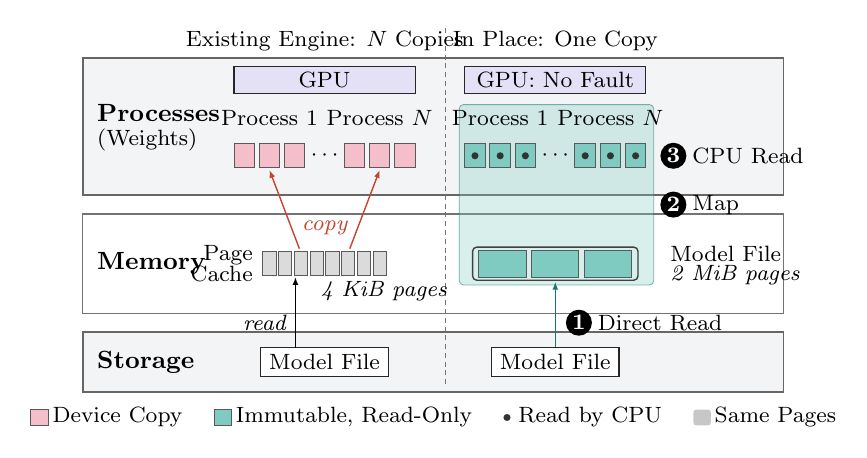
\begin{tikzpicture}[x=1cm, y=1cm,
  tiny/.style={-{Latex[length=1.0mm]}, line width=0.5pt},
  pte/.style={blk, minimum width=0.26cm, minimum height=0.3cm},
  small/.style={blk, minimum width=0.17cm, minimum height=0.3cm, inner xsep=0pt},
  huge/.style={blk, minimum width=0.6cm, minimum height=0.34cm},
  flag/.style={circle, fill=black!80, inner sep=0pt, minimum size=0.09cm}]

% lanes, from the GPU and the processes down to storage
\draw[layer] (0,3.12) rectangle (8.9,4.86);
\draw[sub, fill=white] (0,1.62) rectangle (8.9,2.88);
\draw[layer] (0,0.62) rectangle (8.9,1.38);
\node[ttl, anchor=west, inner sep=1pt] at (0.14,4.16) {Processes};
\node[tag, anchor=west] at (0.14,3.82) {(Weights)};
\node[ttl, anchor=west, inner sep=1pt] at (0.14,2.25) {Memory};
\node[ttl, anchor=west, inner sep=1pt] at (0.14,1.0) {Storage};

% the two designs
\fitdash{4.6}{0.72}{4.6}{5.24}
\node[tag] at (3.07,5.08) {Existing Engine: $N$ Copies};
\node[tag] at (6.0,5.08) {In Place: One Copy};

% a band joins the weight buffers with the pages behind them
\newcommand{\band}[6]{\filldraw[fill=#1, fill opacity=0.3, draw=#6, draw opacity=0.55, line width=0.3pt, rounded corners=1.5pt] (#2,#3) rectangle (#4,#5);}
\band{sharedc}{4.78}{1.98}{7.25}{4.27}{roline}

% ---------------- the existing engine ----------------
\node[comp, fill=gpuc, minimum width=2.3cm, minimum height=0.34cm, inner ysep=0pt] at (3.07,4.58) {GPU};
\node[tag] at (2.37,4.1) {Process 1};
\node[tag] at (3.07,3.62) {$\cdots$};
\node[tag] at (3.77,4.1) {Process $N$};
\foreach \k in {0,1,2} {
  \node[pte, fill=copyc] at (2.05+\k*0.32,3.62) {};
  \node[pte, fill=copyc] at (3.45+\k*0.32,3.62) {};
}
% the page cache, in 4 KiB pages
\foreach \k in {0,...,7} {
  \node[small, fill=black!14] at (2.37+\k*0.2,2.25) {};
}
\node[tag, anchor=east, align=right] at (2.2,2.25) {Page\\[-2pt]Cache};
\node[note, anchor=west] at (2.98,1.9) {4 KiB pages};
\draw[tiny, rwline] (2.75,2.44) -- (2.37,3.44);
\draw[tiny, rwline] (3.39,2.44) -- (3.77,3.44);
\node[note, text=rwline] at (3.07,2.7) {copy};
\node[comp, minimum width=1.5cm, minimum height=0.36cm, inner ysep=0pt] (file0) at (3.07,1.0) {Model File};
\draw[tiny] (2.7,1.18) -- (2.7,2.08);
\node[note, anchor=east] at (2.62,1.5) {read};

% ---------------- the weights in place ----------------
\node[comp, fill=gpuc, minimum width=2.3cm, minimum height=0.34cm, inner ysep=0pt] at (6.0,4.58) {GPU: No Fault};
\node[tag] at (5.3,4.1) {Process 1};
\node[tag] at (6.0,3.62) {$\cdots$};
\node[tag] at (6.7,4.1) {Process $N$};
\foreach \k in {0,1,2} {
  \node[pte, fill=sharedc] (a\k) at (4.98+\k*0.32,3.62) {};
  \node[pte, fill=sharedc] (b\k) at (6.38+\k*0.32,3.62) {};
  \node[flag] at (a\k) {};
  \node[flag] at (b\k) {};
}
% the model file in memory, in 2 MiB pages
\foreach \k in {0,1,2} {
  \node[huge, fill=sharedc] at (5.33+\k*0.67,2.25) {};
}
\draw[black!75, line width=0.5pt, rounded corners=1.5pt] (4.95,2.04) rectangle (7.05,2.46);
\node[tag, anchor=west] at (7.42,2.38) {Model File};
\node[note, anchor=west] at (7.42,2.1) {2 MiB pages};
\node[comp, minimum width=1.5cm, minimum height=0.36cm, inner ysep=0pt] (file1) at (6.0,1.0) {Model File};
\draw[tiny, roline] (file1.north) -- (6.0,2.02);

% the three steps
\node[num] at (6.3,1.5) {1};
\node[tag, anchor=west] at (6.5,1.5) {Direct Read};
\node[num] at (7.5,3.0) {2};
\node[tag, anchor=west] at (7.7,3.0) {Map};
\node[num] at (7.5,3.62) {3};
\node[tag, anchor=west] at (7.7,3.62) {CPU Read};

% legend
\node[tag] at (4.45,0.3) {\lgdfill{copyc}\,Device Copy\quad\ \lgdfill{sharedc}\,Immutable, Read-Only\quad\ \tikz[baseline=-0.55ex]{\node[circle, fill=black!80, inner sep=0pt, minimum size=0.09cm] {};}\,\,Read by CPU\quad\ \tikz[baseline=-0.55ex]{\fill[black!22, rounded corners=1pt] (0,-0.1) rectangle (0.22,0.1);}\,Same Pages};
\end{tikzpicture}
\end{document}
